%!TEX root = ../report.tex
\section{Problem Definition}
% Give a precise formulation of the problem you will be addressing
Since the fluids are simulated using SPH, the fluid is discretized in different particles.
A scene containing a fluid, simulated by SPH, can be seen in figure \ref{..}.
Since this ``fluid'' does not look like a fluid that can be found in nature, a visualization technique has to be applied.

\begin{figure}[!th]
\hrule
\begin{center}
\vspace*{2ex}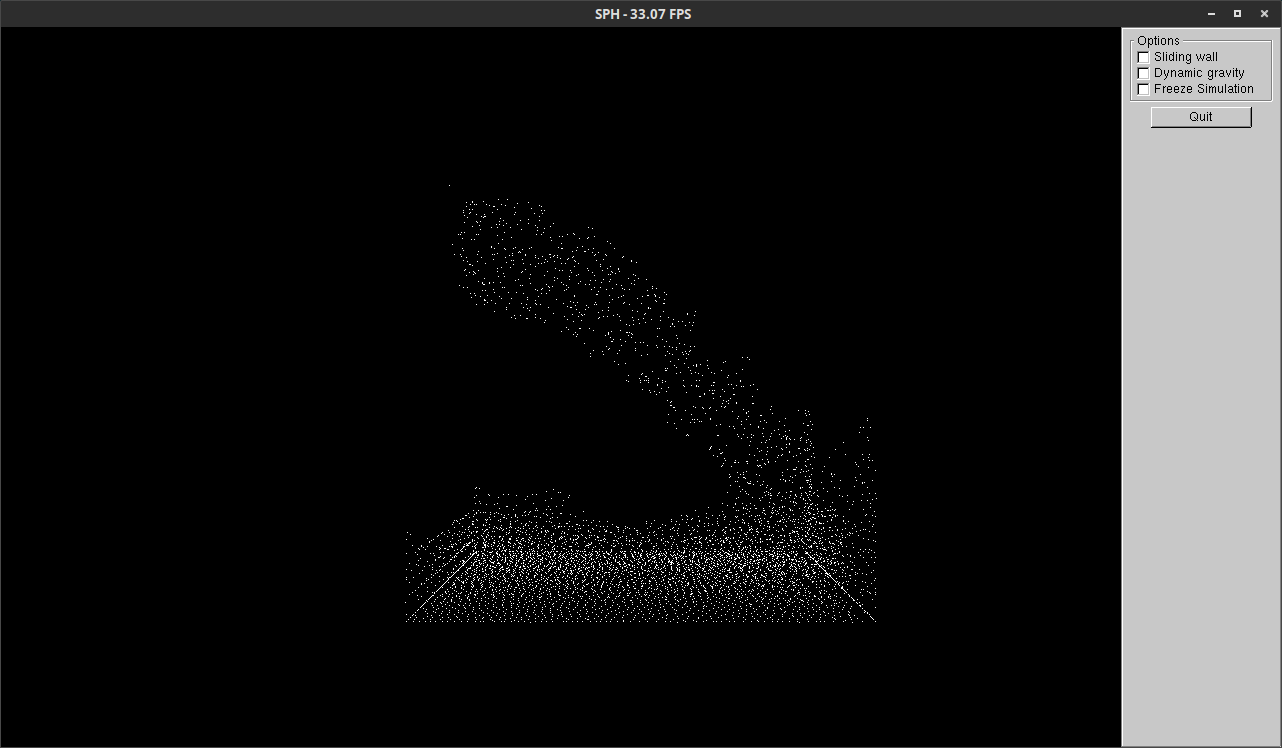
\includegraphics[width=0.48\textwidth]{pictures/sph.png}
\end{center}
\caption{SPH simulation}
\label{fig:sph} 
\vspace*{2ex}
\hrule
\end{figure}

It is our goal to create a nature-like rendering of fluids that can be rendered in real-time, in order to use it in games, for example.
It is also desirable to make sure that the rendering can be customized according to the requirements of users.
For example, fluids can have different kind of thicknesses, or the quality of the rendering can be altered in order to keep the rendering in real-time.

\subsection{Related work}
Various methods are developed that try to achieve a nature-like rendering of fluid.
Some of these techniques require to use a mesh, which is not desirable.
Other techniques have the drawback that they can not be rendered in real-time.

\cite{zhang2008adaptive} developed a method that makes use of point-based rendering, therefore no grid is needed anymore.
However, a drawback of this method is that it results in unreasonably thick surfaces.
